% !TEX root = 0_main.tex
\chapter*{Open Source Logic Synthesis Tools}\label{app:seqos}
\sys{} offers a generic methodology for generating GC that is transparent to the underlying logic synthesis tool.
To show this point, we demonstrate an implementation of \sys{} using the Yosys \cite{tool:Yosys} and ABC \cite{tool:ABC} logic synthesis tool chain for circuit generation.
Both of these tools are open-source and available online.
We compare the performance of the commercial HDL synthesis tool, i.e., Synopsys DC, with this open-source synthesis tool chain.
ABC is an academic package developed at the University of California Berkeley.
Yosys is an HDL-based synthesis tool which calls ABC for its technology mapping.
The HDL inputs for describing both sequential and combinational circuits are written in the Verilog programming language.

We compare the performance of these open-source tools to the commercially available Synopsys DC.
The results are presented in \tab{table:abc}.
For comparison purposes, we compute $\mathit{GTD}$ and $\mathit{MFE}$ using the netlists generated by Synopsys DC as reference.
For most of the benchmarks $\mathit{GTD}$s are either very small or zero which implies that the number of non-XOR gates in circuits generated by Yosys and by Synopsys DC are almost similar.
In terms of memory footprint, different tools perform better for different benchmark functions.
These results shows that \sys{} is transparent to the underlying logic synthesis tool as long as the tool is up to date with respect to the known methods for logic minimization and mapping.
Since the logic synthesis tools perform a series of optimizations, they may use different (heuristic) algorithms for some of their internal steps which could lead to slightly different results.
A user can choose between different synthesis tools based on their performance and availability.

\begin{table}[h]
\caption{Comparison of circuit generation performance between the commercial Synopsys DC and Yosys+ABC open source logic synthesizer.}
\label{table:abc}
\centering
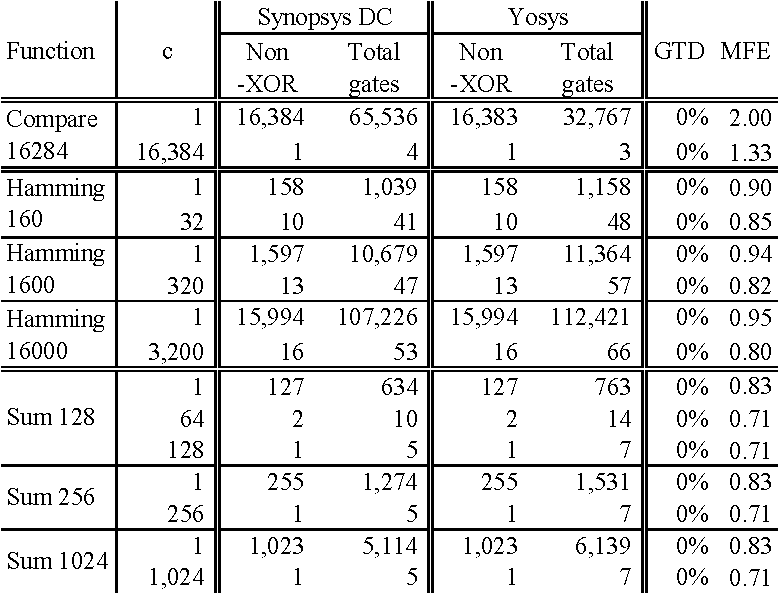
\includegraphics[scale=.9]{abc-crop.pdf}
\end{table}
